\documentclass{standalone}
\usepackage{tikz}
\usepackage{ctex,siunitx}
\usepackage{tkz-euclide}
\usepackage{amsmath}
\usetikzlibrary{patterns, calc}
\usetikzlibrary {decorations.pathmorphing, decorations.pathreplacing, decorations.shapes,}
\begin{document}
\small
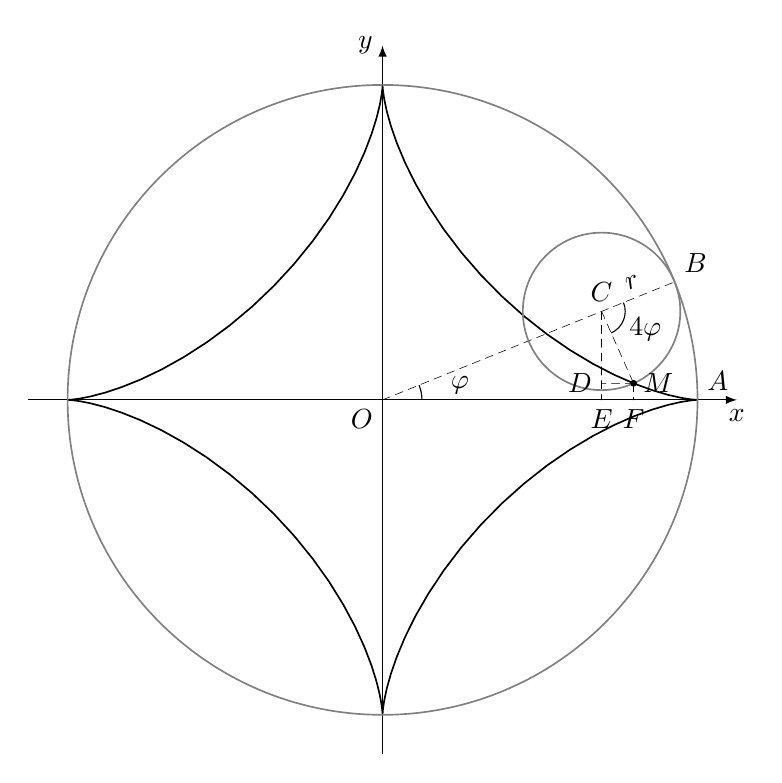
\begin{tikzpicture}[>=latex,scale=1]
  \draw[thin,->](-4.5,0)--(4.5,0)node[below]{$x$};
  \draw[thin,->](0,-4.5)--(0,4.5)node[left]{$y$};
  \tkzDefPoints{0/0/O,4/0/A}
  \tkzDefShiftPoint[O](22:3){C}
  \tkzDefShiftPoint[O](22:4){B}
  \tkzDefShiftPoint[C](-66:1){M}
  \tkzDefPointBy[projection=onto O--A](C)\tkzGetPoint{E}
  \tkzDefPointBy[projection=onto O--A](M)\tkzGetPoint{F}
  \tkzDefPointBy[projection=onto C--E](M)\tkzGetPoint{D}
  \draw[semithick,domain=0:360,samples=100] plot ({4*cos(\x)*cos(\x)*cos(\x)},{4*sin(\x)*sin(\x)*sin(\x)});
  \tkzLabelLine[pos=0.5,sloped,above](C,B){$r$}
  \tkzDrawSegments[densely dashed](C,M C,E O,B M,D M,F)
  \tkzDrawCircle[semithick](O,A)
  \tkzDrawCircle[semithick](C,B)
  \tkzDrawPoints[fill=black](M)
  \tkzMarkAngle[size=0.5](A,O,B)
  \tkzLabelAngle[pos=1.0](A,O,B){$\varphi$}
  \tkzMarkAngle[size=0.3](M,C,B)
  \tkzLabelAngle[pos=0.6](M,C,B){$4\varphi$}
  \tkzLabelPoints[left](D)
  \tkzLabelPoints[right](M)
  \tkzLabelPoints[above](C)
  \tkzLabelPoints(E,F)
  \tkzLabelPoints[above right](A,B)
  \tkzLabelPoints[below left](O)
\end{tikzpicture}
\end{document}